\subsection{UC1: Comunicazione nome e cognome}
\label{UC1}
\begin{longtable}{l|p{10cm}}
\rowcolor[gray]{0.8} \multicolumn{2}{c}{} \\
\rowcolor[gray]{0.8} \multicolumn{2}{c}{\textbf{UC1 - Comunicazione nome e cognome}} \\
\rowcolor[gray]{0.8} \multicolumn{2}{c}{} \\
\hline
&\\
\textbf{Attori} & Utente.\\[7pt]
\textbf{Descrizione} & Il sistema deve permettere all'utente di fornire il proprio nome e cognome per essere identificato.\\[7pt]
\textbf{Precondizione} & Il sistema è pronto e in attesa di ricevere nome e cognome da parte dell'utente.\\[7pt]
\textbf{Postcondizione} & Il sistema ha ottenuto nome e cognome dell'utente.\\[7pt]
\textbf{Scenario principale} &L'utente comunica il proprio nome e cognome. \\[7pt]\hline
\end{longtable}

\newpage\subsection{UC2: Accesso funzionalità amministratore}
\label{UC2}
\begin{figure}[h]
\centering
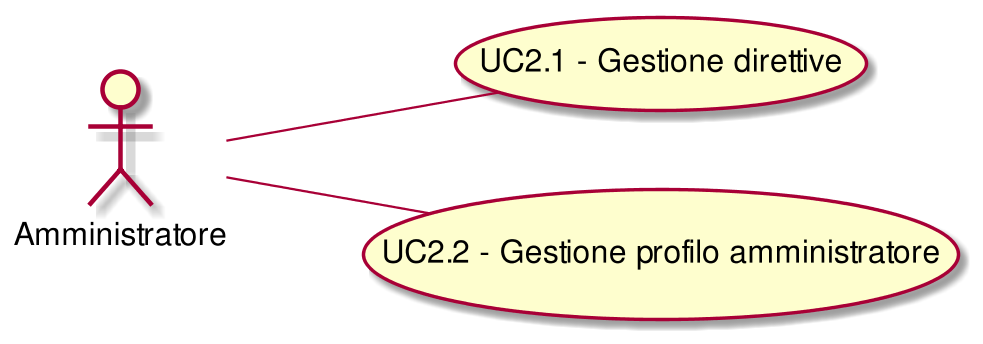
\includegraphics[width=\textwidth,height=\textheight,keepaspectratio]{images/UseCaseUC2.png}
\caption{UC2: Accesso funzionalità amministratore}
\end{figure}
\begin{longtable}{l|p{10cm}}
\rowcolor[gray]{0.8} \multicolumn{2}{c}{} \\
\rowcolor[gray]{0.8} \multicolumn{2}{c}{\textbf{UC2 - Accesso funzionalità amministratore}} \\
\rowcolor[gray]{0.8} \multicolumn{2}{c}{} \\
\hline
&\\
\textbf{Attori} & Amministratore.\\[7pt]
\textbf{Descrizione} & L'amministratore deve poter accedere alle funzionalità avanzate messe a disposizione dall'applicazione. Tali funzionalità consentono di fornire delle direttive per l'interazione con gli ospiti al sistema.\\[7pt]
\textbf{Precondizione} & L'amministratore ha effettuato l'accesso tramite la password di amministrazione.\\[7pt]
\textbf{Postcondizione} & L'amministratore ha usufruito delle funzionalità di amministratore.\\[7pt]
\textbf{Scenario principale} &\begin{enumerate}
\item  L'amministratore può gestire le direttive del sistema da lui accessibili;
\item  L'amministratore può gestire le informazioni del proprio profilo.
\end{enumerate}
\\[7pt]\hline
\end{longtable}

\newpage\subsubsection{UC2.1: Gestione direttive}
\label{UC2.1}
\begin{figure}[h]
\centering
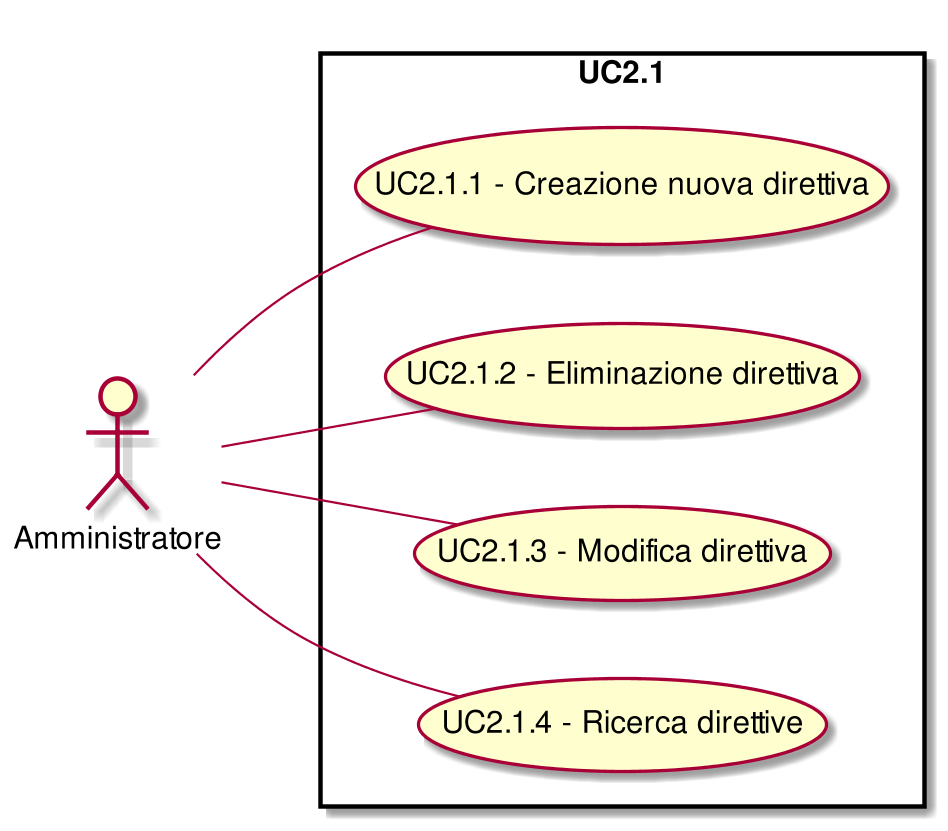
\includegraphics[width=\textwidth,height=\textheight,keepaspectratio]{images/UseCaseUC21.png}
\caption{UC2.1: Gestione direttive}
\end{figure}
\begin{longtable}{l|p{10cm}}
\rowcolor[gray]{0.8} \multicolumn{2}{c}{} \\
\rowcolor[gray]{0.8} \multicolumn{2}{c}{\textbf{UC2.1 - Gestione direttive}} \\
\rowcolor[gray]{0.8} \multicolumn{2}{c}{} \\
\hline
&\\
\textbf{Attori} & Amministratore.\\[7pt]
\textbf{Descrizione} & L'amministratore può gestire le direttive da lui accessibili.\\[7pt]
\textbf{Precondizione} & L'amministratore si trova nella sezione adibita alla gestione delle direttive.\\[7pt]
\textbf{Postcondizione} & L'amministratore ha usufruito delle funzionalità per gestire le direttive.\\[7pt]
\textbf{Scenario principale} &\begin{enumerate}
\item  L'amministratore può creare una nuova direttiva;
\item  L'amministratore può eliminare una direttiva da lui accessibile;
\item  L'amministratore può modificare una direttiva da lui accessibile;
\item  L'amministratore può filtrare la lista delle direttive da lui accessibili in diversi modi;
\item  L'amministratore può ordinare la lista delle direttive da lui accessibili in diversi modi.
\end{enumerate}
\\[7pt]\hline
\end{longtable}

\newpage
\subsubsection{UC2.1.1: Creazione nuova direttiva}
\label{UC2.1.1}
\begin{figure}[h]
\centering
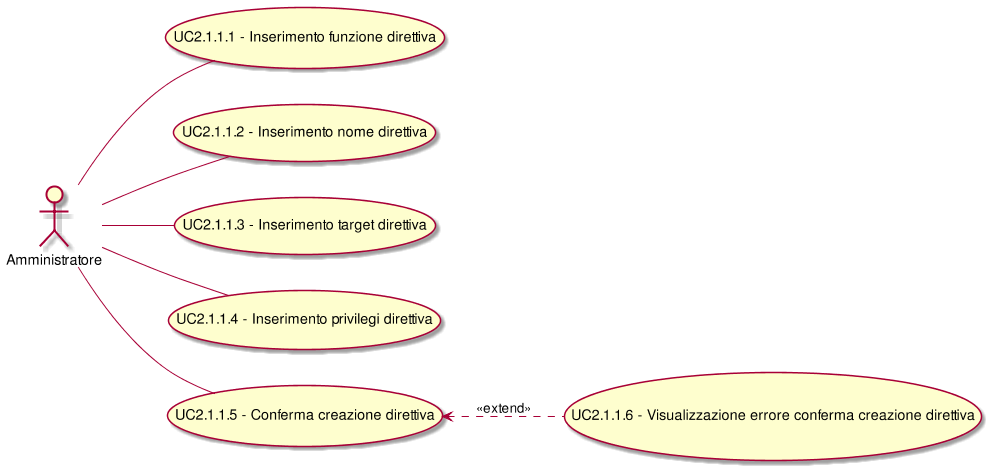
\includegraphics[width=\textwidth,height=\textheight,keepaspectratio]{images/UseCaseUC211.png}
\caption{UC2.1.1: Creazione nuova direttiva}
\end{figure}
\begin{longtable}{l|p{10cm}}
\rowcolor[gray]{0.8} \multicolumn{2}{c}{} \\
\rowcolor[gray]{0.8} \multicolumn{2}{c}{\textbf{UC2.1.1 - Creazione nuova direttiva}} \\
\rowcolor[gray]{0.8} \multicolumn{2}{c}{} \\
\hline
&\\
\textbf{Attori} & Amministratore.\\[7pt]
\textbf{Descrizione} & L'amministratore può creare una nuova direttiva, la quale sarà salvata nel sistema.\\[7pt]
\textbf{Precondizione} & L'amministratore si trova nella sezione dedicata alla creazione di una nuova direttiva.\\[7pt]
\textbf{Postcondizione} & La direttiva è stata creata e salvata nel sistema.\\[7pt]
\textbf{Scenario principale} &\begin{enumerate}
\item  L'amministratore può inserire il nome della direttiva;
\item  L'amministratore può inserire il target della direttiva;
\item  L'amministratore può inserire la funzione della direttiva;
\item  L'amministratore può confermare la creazione della direttiva. 
\end{enumerate}
\\[7pt]
\textbf{Scenari alternativi} & L'amministratore visualizza un messaggio d'errore relativo alla conferma della creazione della direttiva.\\[7pt]\hline
\end{longtable}

\subsubsection{UC2.1.1.1: Inserimento funzione direttiva}
\label{UC2.1.1.1}
\begin{longtable}{l|p{10cm}}
\rowcolor[gray]{0.8} \multicolumn{2}{c}{} \\
\rowcolor[gray]{0.8} \multicolumn{2}{c}{\textbf{UC2.1.1.1 - Inserimento funzione direttiva}} \\
\rowcolor[gray]{0.8} \multicolumn{2}{c}{} \\
\hline
&\\
\textbf{Attori} & Amministratore.\\[7pt]
\textbf{Descrizione} & L'amministratore può inserire la funzione di una direttiva.\\[7pt]
\textbf{Precondizione} & L'amministratore si trova nella sezione dedicata all'inserimento della funzione di una direttiva.\\[7pt]
\textbf{Postcondizione} & L'amministratore ha inserito la funzione di una direttiva.\\[7pt]
\textbf{Scenario principale} &L'amministratore inserisce la funzione di una direttiva.\\[7pt]\hline
\end{longtable}

\subsubsection{UC2.1.1.2: Inserimento nome direttiva}
\label{UC2.1.1.2}
\begin{longtable}{l|p{10cm}}
\rowcolor[gray]{0.8} \multicolumn{2}{c}{} \\
\rowcolor[gray]{0.8} \multicolumn{2}{c}{\textbf{UC2.1.1.2 - Inserimento nome direttiva}} \\
\rowcolor[gray]{0.8} \multicolumn{2}{c}{} \\
\hline
&\\
\textbf{Attori} & Amministratore.\\[7pt]
\textbf{Descrizione} & L'amministratore può inserire il nome di una direttiva.\\[7pt]
\textbf{Precondizione} & L'amministratore si trova nella sezione dedicata all'inserimento del nome di una direttiva.\\[7pt]
\textbf{Postcondizione} & L'amministratore ha inserito il nome di una direttiva.\\[7pt]
\textbf{Scenario principale} &L'amministratore inserisce il nome di una direttiva.\\[7pt]\hline
\end{longtable}

\subsubsection{UC2.1.1.3: Inserimento target direttiva}
\label{UC2.1.1.3}
\begin{longtable}{l|p{10cm}}
\rowcolor[gray]{0.8} \multicolumn{2}{c}{} \\
\rowcolor[gray]{0.8} \multicolumn{2}{c}{\textbf{UC2.1.1.3 - Inserimento target direttiva}} \\
\rowcolor[gray]{0.8} \multicolumn{2}{c}{} \\
\hline
&\\
\textbf{Attori} & Amministratore.\\[7pt]
\textbf{Descrizione} & L'amministratore può inserire il target di una direttiva.\\[7pt]
\textbf{Precondizione} & L'amministratore si trova nella sezione dedicata all'inserimento dei target di una direttiva.\\[7pt]
\textbf{Postcondizione} & L'amministratore ha inserito i target di una direttiva.\\[7pt]
\textbf{Scenario principale} &L'amministratore inserisce i target di una direttiva.\\[7pt]\hline
\end{longtable}

\subsubsection{UC2.1.1.4: Inserimento privilegi direttiva}
\label{UC2.1.1.4}
\begin{longtable}{l|p{10cm}}
\rowcolor[gray]{0.8} \multicolumn{2}{c}{} \\
\rowcolor[gray]{0.8} \multicolumn{2}{c}{\textbf{UC2.1.1.4 - Inserimento privilegi direttiva}} \\
\rowcolor[gray]{0.8} \multicolumn{2}{c}{} \\
\hline
&\\
\textbf{Attori} & Amministratore.\\[7pt]
\textbf{Descrizione} & L'amministratore può concedere i privilegi per la direttiva ad altri amministratori.\\[7pt]
\textbf{Precondizione} & L'amministratore si trova nella sezione relativa all'inserimento dei privilegi per la direttiva\\[7pt]
\textbf{Postcondizione} & L'amministratore ha inserito i privilegi per la direttiva\\[7pt]
\textbf{Scenario principale} &L'amministratore specifica chi tra gliu altri amministratori può accedere alla direttiva e può modificarla.\\[7pt]\hline
\end{longtable}

\subsubsection{UC2.1.1.5: Conferma creazione direttiva}
\label{UC2.1.1.5}
\begin{longtable}{l|p{10cm}}
\rowcolor[gray]{0.8} \multicolumn{2}{c}{} \\
\rowcolor[gray]{0.8} \multicolumn{2}{c}{\textbf{UC2.1.1.5 - Conferma creazione direttiva}} \\
\rowcolor[gray]{0.8} \multicolumn{2}{c}{} \\
\hline
&\\
\textbf{Attori} & Amministratore.\\[7pt]
\textbf{Descrizione} & L'amministratore può confermare la creazione di una nuova direttiva.\\[7pt]
\textbf{Precondizione} & L'amministratore ha inserito i dati necessari alla creazione di una direttiva.\\[7pt]
\textbf{Postcondizione} & L'amministratore ha creato una nuova direttiva.\\[7pt]
\textbf{Scenario principale} &L'amministratore conferma di voler creare la nuova direttiva.\\[7pt]
\textbf{Scenari alternativi} & L'amministratore non conferma di voler creare la direttiva. L'amministratore viene rimandato alla pagina dedicata alla gestione delle direttive.\\[7pt]\hline
\end{longtable}

\subsubsection{UC2.1.1.6: Visualizzazione errore conferma creazione direttiva}
\label{UC2.1.1.6}
\begin{longtable}{l|p{10cm}}
\rowcolor[gray]{0.8} \multicolumn{2}{c}{} \\
\rowcolor[gray]{0.8} \multicolumn{2}{c}{\textbf{UC2.1.1.6 - Visualizzazione errore conferma creazione direttiva}} \\
\rowcolor[gray]{0.8} \multicolumn{2}{c}{} \\
\hline
&\\
\textbf{Attori} & Amministratore.\\[7pt]
\textbf{Descrizione} & L'amministratore può visualizzare un messaggio d'errore se ha comunicato dei dati nulli o non validi per la creazione di una nuova direttiva.\\[7pt]
\textbf{Precondizione} & Il sistema ha ricevuto dati vuoti o non validi.\\[7pt]
\textbf{Postcondizione} & Il sistema mostra un messaggio d'errore.\\[7pt]
\textbf{Scenario principale} &L'amministratore visualizza un messaggio d'errore.\\[7pt]\hline
\end{longtable}

\newpage\subsubsection{UC2.1.2: Eliminazione direttiva }
\label{UC2.1.2}
\begin{figure}[h]
\centering
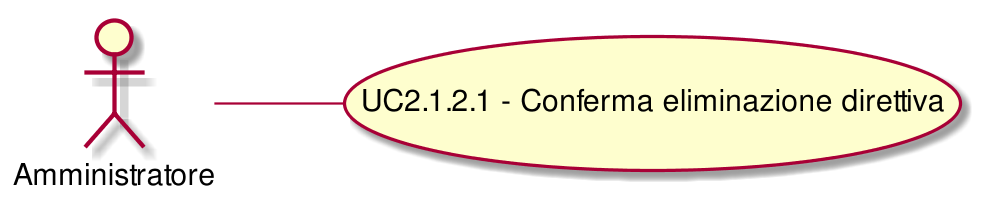
\includegraphics[width=\textwidth,height=\textheight,keepaspectratio]{images/UseCaseUC212.png}
\caption{UC2.1.2: Eliminazione direttiva }
\end{figure}
\begin{longtable}{l|p{10cm}}
\rowcolor[gray]{0.8} \multicolumn{2}{c}{} \\
\rowcolor[gray]{0.8} \multicolumn{2}{c}{\textbf{UC2.1.2 - Eliminazione direttiva }} \\
\rowcolor[gray]{0.8} \multicolumn{2}{c}{} \\
\hline
&\\
\textbf{Attori} & Amministratore.\\[7pt]
\textbf{Descrizione} & L'amministratore può eliminare dal sistema una direttiva di cui ha i privilegi. L'eliminazione comporterà la cancellazione dei dati dal sistema.\\[7pt]
\textbf{Precondizione} & L'amministratore si trova nella sezione dedicata alla eliminazione di una direttiva.\\[7pt]
\textbf{Postcondizione} & La direttiva è stata rimossa dal sistema.\\[7pt]
\textbf{Scenario principale} &L'amministratore può confermare di voler eliminare una direttiva.\\[7pt]\hline
\end{longtable}

\subsubsection{UC2.1.2.1: Conferma eliminazione direttiva}
\label{UC2.1.2.1}
\begin{longtable}{l|p{10cm}}
\rowcolor[gray]{0.8} \multicolumn{2}{c}{} \\
\rowcolor[gray]{0.8} \multicolumn{2}{c}{\textbf{UC2.1.2.1 - Conferma eliminazione direttiva}} \\
\rowcolor[gray]{0.8} \multicolumn{2}{c}{} \\
\hline
&\\
\textbf{Attori} & Amministratore.\\[7pt]
\textbf{Descrizione} & L'amministratore può confermare l'eliminazione di una direttiva.\\[7pt]
\textbf{Precondizione} & L'amministratore ha comunicato i dati necessari per l'eliminazione di una direttiva.\\[7pt]
\textbf{Postcondizione} & L'amministratore ha eliminato una direttiva.\\[7pt]
\textbf{Scenario principale} &L'amministratore conferma di voler eliminare la direttiva.\\[7pt]
\textbf{Scenari alternativi} & L'amministratore non conferma di voler eliminare la direttiva. L'amministratore viene rimandato alla pagina dedicata alla gestione delle direttive.\\[7pt]\hline
\end{longtable}

\newpage\subsubsection{UC2.1.3: Modifica direttiva}
\label{UC2.1.3}
\begin{figure}[h]
\centering
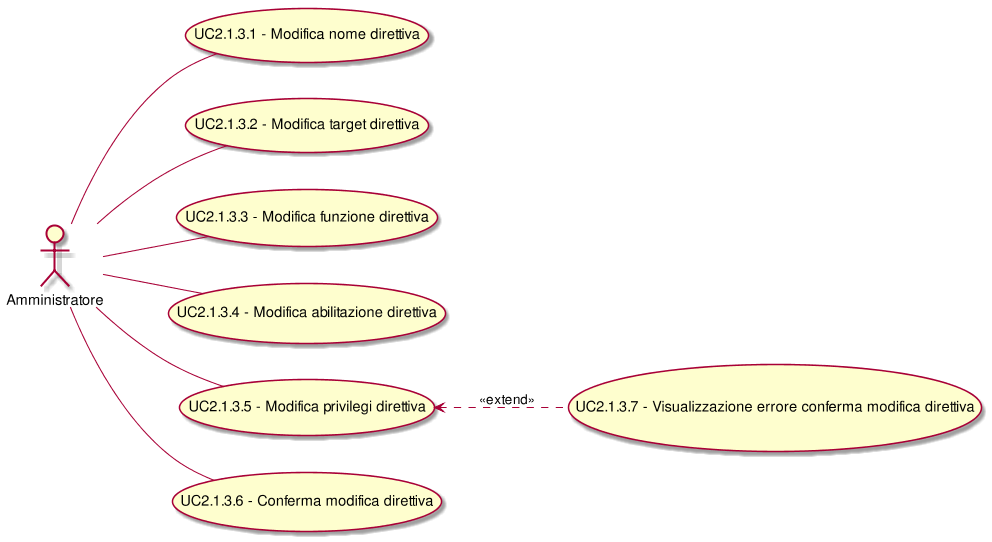
\includegraphics[width=\textwidth,height=\textheight,keepaspectratio]{images/UseCaseUC213.png}
\caption{UC2.1.3: Modifica direttiva}
\end{figure}
\begin{longtable}{l|p{10cm}}
\rowcolor[gray]{0.8} \multicolumn{2}{c}{} \\
\rowcolor[gray]{0.8} \multicolumn{2}{c}{\textbf{UC2.1.3 - Modifica direttiva}} \\
\rowcolor[gray]{0.8} \multicolumn{2}{c}{} \\
\hline
&\\
\textbf{Attori} & Amministratore.\\[7pt]
\textbf{Descrizione} & L'amministratore può modificare una direttiva di cui ha i privilegi. \\[7pt]
\textbf{Precondizione} & L'amministratore si trova nella sezione dedicata alla modifica delle direttive.\\[7pt]
\textbf{Postcondizione} & L'amministratore ha modificato la direttiva selezionata.\\[7pt]
\textbf{Scenario principale} &\begin{enumerate}
\item  L'amministratore può modificare il nome della direttiva;
\item  L'amministratore può modificare il target della direttiva;
\item  L'amministratore può modificare la funzione della direttiva;
\item  L'amministratore può abilitare o disabilitare una direttiva;
\item  L'amministratore può confermare le modifiche apportate alla direttiva.
\end{enumerate}
\\[7pt]
\textbf{Scenari alternativi} & L'amministratore visualizza un messaggio d'errore relativo alla modifica della direttiva.\\[7pt]\hline
\end{longtable}

\newpage
\subsubsection{UC2.1.3.1: Modifica nome direttiva}
\label{UC2.1.3.1}
\begin{longtable}{l|p{10cm}}
\rowcolor[gray]{0.8} \multicolumn{2}{c}{} \\
\rowcolor[gray]{0.8} \multicolumn{2}{c}{\textbf{UC2.1.3.1 - Modifica nome direttiva}} \\
\rowcolor[gray]{0.8} \multicolumn{2}{c}{} \\
\hline
&\\
\textbf{Attori} & Amministratore.\\[7pt]
\textbf{Descrizione} & L'amministratore può modificare il nome di una direttiva.\\[7pt]
\textbf{Precondizione} & L'amministratore si trova nella sezione dedicata alla modifica del nome di una direttiva.\\[7pt]
\textbf{Postcondizione} & L'amministratore ha modificato il nome di una direttiva.\\[7pt]
\textbf{Scenario principale} &L'amministratore modifica il nome di una direttiva.\\[7pt]\hline
\end{longtable}

\subsubsection{UC2.1.3.2: Modifica target direttiva}
\label{UC2.1.3.2}
\begin{longtable}{l|p{10cm}}
\rowcolor[gray]{0.8} \multicolumn{2}{c}{} \\
\rowcolor[gray]{0.8} \multicolumn{2}{c}{\textbf{UC2.1.3.2 - Modifica target direttiva}} \\
\rowcolor[gray]{0.8} \multicolumn{2}{c}{} \\
\hline
&\\
\textbf{Attori} & Amministratore.\\[7pt]
\textbf{Descrizione} & L'amministratore può modificare i target di una direttiva.\\[7pt]
\textbf{Precondizione} & L'amministratore si trova nella sezione dedicata alla modifica dei target di una direttiva.\\[7pt]
\textbf{Postcondizione} & L'amministratore ha modificato i target di una direttiva.\\[7pt]
\textbf{Scenario principale} &L'amministratore modifica i target di una direttiva.\\[7pt]\hline
\end{longtable}

\subsubsection{UC2.1.3.3: Modifica funzione direttiva}
\label{UC2.1.3.3}
\begin{longtable}{l|p{10cm}}
\rowcolor[gray]{0.8} \multicolumn{2}{c}{} \\
\rowcolor[gray]{0.8} \multicolumn{2}{c}{\textbf{UC2.1.3.3 - Modifica funzione direttiva}} \\
\rowcolor[gray]{0.8} \multicolumn{2}{c}{} \\
\hline
&\\
\textbf{Attori} & Amministratore.\\[7pt]
\textbf{Descrizione} & L'amministratore può modificare la funzione di una direttiva.\\[7pt]
\textbf{Precondizione} & L'amministratore si trova nella sezione dedicata alla modifica della funzione di una direttiva.\\[7pt]
\textbf{Postcondizione} & L'amministratore ha modificato la funzione di una direttiva.\\[7pt]
\textbf{Scenario principale} &L'amministratore modifica la funzione di una direttiva.\\[7pt]\hline
\end{longtable}

\newpage
\subsubsection{UC2.1.3.4: Modifica abilitazione direttiva}
\label{UC2.1.3.4}
\begin{longtable}{l|p{10cm}}
\rowcolor[gray]{0.8} \multicolumn{2}{c}{} \\
\rowcolor[gray]{0.8} \multicolumn{2}{c}{\textbf{UC2.1.3.4 - Modifica abilitazione direttiva}} \\
\rowcolor[gray]{0.8} \multicolumn{2}{c}{} \\
\hline
&\\
\textbf{Attori} & Amministratore.\\[7pt]
\textbf{Descrizione} & L'amministratore può modificare l'abilitazione di una direttiva.\\[7pt]
\textbf{Precondizione} & L'amministratore si trova nella sezione dedicata all'abilitazione di una direttiva.\\[7pt]
\textbf{Postcondizione} & L'amministratore ha modificato l'abilitazione di una direttiva.\\[7pt]
\textbf{Scenario principale} &L'amministratore modifica l'abilitazione di una direttiva\\[7pt]\hline
\end{longtable}

\subsubsection{UC2.1.3.5: Modifica privilegi direttiva}
\label{UC2.1.3.5}
\begin{figure}[h]
\centering
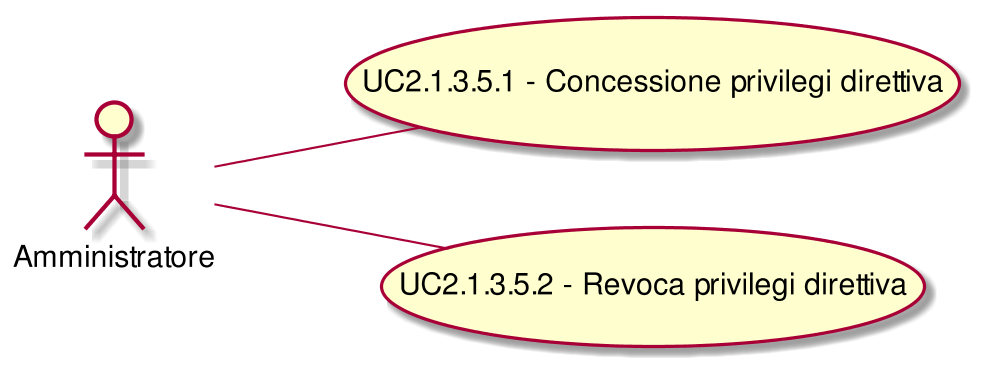
\includegraphics[width=\textwidth,height=\textheight,keepaspectratio]{images/UseCaseUC2135.png}
\caption{UC2.1.3.5: Modifica privilegi direttiva}
\end{figure}
\begin{longtable}{l|p{10cm}}
\rowcolor[gray]{0.8} \multicolumn{2}{c}{} \\
\rowcolor[gray]{0.8} \multicolumn{2}{c}{\textbf{UC2.1.3.5 - Modifica privilegi direttiva}} \\
\rowcolor[gray]{0.8} \multicolumn{2}{c}{} \\
\hline
&\\
\textbf{Attori} & Amministratore.\\[7pt]
\textbf{Descrizione} & L'amministratore può modificare i privilegi degli altri amministratori per la direttiva.\\[7pt]
\textbf{Precondizione} & L'amministratore si trova nella sezione dedicata alla modifica dei privilegi degli altri amministratori per una direttiva.\\[7pt]
\textbf{Postcondizione} & L'amministratore ha modificato i privilegi degli altri amministratori per una direttiva.\\[7pt]
\textbf{Scenario principale} &\begin{enumerate}
\item  L'amministratore può concedere ad un altro amministratore i privilegi per una direttiva;
\item  L'amministratore può revocare i privilegi di un altro amministratore per una direttiva.
\end{enumerate}
\\[7pt]\hline
\end{longtable}

\subsubsection{UC2.1.3.5.1: Concessione privilegi direttiva}
\label{UC2.1.3.5.1}
\begin{longtable}{l|p{10cm}}
\rowcolor[gray]{0.8} \multicolumn{2}{c}{} \\
\rowcolor[gray]{0.8} \multicolumn{2}{c}{\textbf{UC2.1.3.5.1 - Concessione privilegi direttiva}} \\
\rowcolor[gray]{0.8} \multicolumn{2}{c}{} \\
\hline
&\\
\textbf{Attori} & Amministratore.\\[7pt]
\textbf{Descrizione} & L'amministratore può concedere ad altri amministratori i privilegi per la direttiva. L'altro amministratore in seguito potrà visualizzare, modificare ed eliminare la direttiva\\[7pt]
\textbf{Precondizione} & L'amministratore si trova nella sezione dedicata alla concessione dei privilegi per la direttiva\\[7pt]
\textbf{Postcondizione} & L'amministratore ha concesso i privilegi per la direttiva ad un altro amministratore\\[7pt]
\textbf{Scenario principale} &L'amministratore concede i privilegi per la direttiva ad un altro amministratore\\[7pt]\hline
\end{longtable}

\subsubsection{UC2.1.3.5.2: Revoca privilegi direttiva}
\label{UC2.1.3.5.2}
\begin{longtable}{l|p{10cm}}
\rowcolor[gray]{0.8} \multicolumn{2}{c}{} \\
\rowcolor[gray]{0.8} \multicolumn{2}{c}{\textbf{UC2.1.3.5.2 - Revoca privilegi direttiva}} \\
\rowcolor[gray]{0.8} \multicolumn{2}{c}{} \\
\hline
&\\
\textbf{Attori} & Amministratore.\\[7pt]
\textbf{Descrizione} & L'amministratore può revocare i privilegi degli altri amministratori per la direttiva.\\[7pt]
\textbf{Precondizione} & L'amministratore si trova nella sezione dedicata alla revoca dei privilegi per una direttiva.\\[7pt]
\textbf{Postcondizione} & L'amministratore ha revocato i privilegi per una direttiva a un altro amministratore.\\[7pt]
\textbf{Scenario principale} &L'amministratore revoca i privilegi per la direttiva ad un altro amministratore.\\[7pt]\hline
\end{longtable}

\subsubsection{UC2.1.3.6: Conferma modifica direttiva}
\label{UC2.1.3.6}
\begin{longtable}{l|p{10cm}}
\rowcolor[gray]{0.8} \multicolumn{2}{c}{} \\
\rowcolor[gray]{0.8} \multicolumn{2}{c}{\textbf{UC2.1.3.6 - Conferma modifica direttiva}} \\
\rowcolor[gray]{0.8} \multicolumn{2}{c}{} \\
\hline
&\\
\textbf{Attori} & Amministratore.\\[7pt]
\textbf{Descrizione} & L'amministratore può confermare la modifica di una direttiva.\\[7pt]
\textbf{Precondizione} & L'amministratore ha inserito i dati necessari alla modifica di una direttiva.\\[7pt]
\textbf{Postcondizione} & L'amministratore ha modificato una direttiva.\\[7pt]
\textbf{Scenario principale} &L'amministratore conferma di voler modificare una direttiva.\\[7pt]
\textbf{Scenari alternativi} & L'amministratore non conferma di voler modificare la direttiva. L'amministratore viene rimandato alla pagina dedicata alla gestione delle direttive.\\[7pt]\hline
\end{longtable}

\subsubsection{UC2.1.3.7: Visualizzazione errore conferma modifica direttiva}
\label{UC2.1.3.7}
\begin{longtable}{l|p{10cm}}
\rowcolor[gray]{0.8} \multicolumn{2}{c}{} \\
\rowcolor[gray]{0.8} \multicolumn{2}{c}{\textbf{UC2.1.3.7 - Visualizzazione errore conferma modifica direttiva}} \\
\rowcolor[gray]{0.8} \multicolumn{2}{c}{} \\
\hline
&\\
\textbf{Attori} & Amministratore.\\[7pt]
\textbf{Descrizione} & L'amministratore può visualizzare un messaggio d'errore se ha comunicato dei dati nulli o non validi per la modifica di una direttiva.\\[7pt]
\textbf{Precondizione} & Il sistema ha ricevuto dati vuoti o non validi.\\[7pt]
\textbf{Postcondizione} & Il sistema mostra un messaggio d'errore.\\[7pt]
\textbf{Scenario principale} &L'amministratore visualizza un messaggio d'errore.\\[7pt]\hline
\end{longtable}

\newpage\subsubsection{UC2.1.4: Visualizzazione direttive }
\label{UC2.1.4}
\begin{figure}[h]
\centering
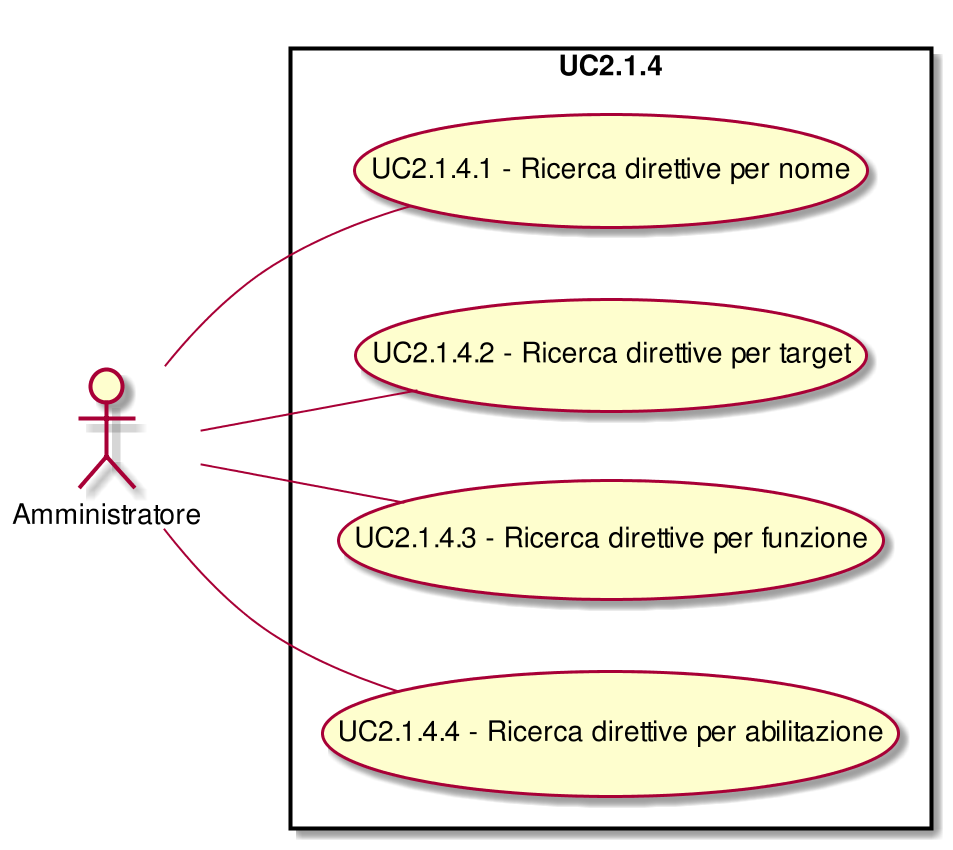
\includegraphics[width=\textwidth,height=\textheight,keepaspectratio]{images/UseCaseUC214.png}
\caption{UC2.1.4: Visualizzazione direttive }
\end{figure}
\begin{longtable}{l|p{10cm}}
\rowcolor[gray]{0.8} \multicolumn{2}{c}{} \\
\rowcolor[gray]{0.8} \multicolumn{2}{c}{\textbf{UC2.1.4 - Visualizzazione direttive }} \\
\rowcolor[gray]{0.8} \multicolumn{2}{c}{} \\
\hline
&\\
\textbf{Attori} & Amministratore.\\[7pt]
\textbf{Descrizione} & L'amministratore può visualizzare tutte le direttive da lui accessibili.\\[7pt]
\textbf{Precondizione} & L'amministratore si trova nella sezione dedicata alla visualizzazione delle direttive.\\[7pt]
\textbf{Postcondizione} & L'amministratore ha visualizzato le direttive da lui cercate.\\[7pt]
\textbf{Scenario principale} &\begin{enumerate}
\item  L'amministratore può cercare le direttive in base al loro nome;
\item  L'amministratore può cercare le direttive in base al loro target;
\item  L'amministratore può cercare le direttive in base alla loro funzione;
\item  L'amministratore può cercare le direttive in base al loro stato di abilitazione.
\end{enumerate}
\\[7pt]\hline
\end{longtable}

\subsubsection{UC2.1.4.1: Ricerca direttive per nome}
\label{UC2.1.4.1}
\begin{longtable}{l|p{10cm}}
\rowcolor[gray]{0.8} \multicolumn{2}{c}{} \\
\rowcolor[gray]{0.8} \multicolumn{2}{c}{\textbf{UC2.1.4.1 - Ricerca direttive per nome}} \\
\rowcolor[gray]{0.8} \multicolumn{2}{c}{} \\
\hline
&\\
\textbf{Attori} & Amministratore.\\[7pt]
\textbf{Descrizione} & L'amministratore può cercare delle direttive in base al nome.\\[7pt]
\textbf{Precondizione} & L'amministratore si trova nella sezione dedicata alla ricerca delle direttive.\\[7pt]
\textbf{Postcondizione} & L'amministratore ha cercato delle direttive in base al nome.\\[7pt]
\textbf{Scenario principale} &L'amministratore cerca delle direttive in base al nome.\\[7pt]\hline
\end{longtable}

\subsubsection{UC2.1.4.2: Ricerca direttive per target}
\label{UC2.1.4.2}
\begin{longtable}{l|p{10cm}}
\rowcolor[gray]{0.8} \multicolumn{2}{c}{} \\
\rowcolor[gray]{0.8} \multicolumn{2}{c}{\textbf{UC2.1.4.2 - Ricerca direttive per target}} \\
\rowcolor[gray]{0.8} \multicolumn{2}{c}{} \\
\hline
&\\
\textbf{Attori} & Amministratore.\\[7pt]
\textbf{Descrizione} & L'amministratore può cercare delle direttive in base ai target.\\[7pt]
\textbf{Precondizione} & L'amministratore si trova nella sezione dedicata alla ricerca delle direttive.\\[7pt]
\textbf{Postcondizione} & L'amministratore ha cercato delle direttive in base ai target\\[7pt]
\textbf{Scenario principale} &L'amministratore cerca delle direttive in base ai target.\\[7pt]\hline
\end{longtable}

\subsubsection{UC2.1.4.3: Ricerca direttive per funzione}
\label{UC2.1.4.3}
\begin{longtable}{l|p{10cm}}
\rowcolor[gray]{0.8} \multicolumn{2}{c}{} \\
\rowcolor[gray]{0.8} \multicolumn{2}{c}{\textbf{UC2.1.4.3 - Ricerca direttive per funzione}} \\
\rowcolor[gray]{0.8} \multicolumn{2}{c}{} \\
\hline
&\\
\textbf{Attori} & Amministratore.\\[7pt]
\textbf{Descrizione} & L'amministratore può cercare le direttive in base alla loro funzione.\\[7pt]
\textbf{Precondizione} & L'amministratore si trova nella sezione dedicata alla ricerca delle direttive.\\[7pt]
\textbf{Postcondizione} & L'amministratore ha cercato e visualizzato le direttive in base alla loro funzione.\\[7pt]
\textbf{Scenario principale} &L'amministratore cerca le direttive in base alla loro funzione.\\[7pt]\hline
\end{longtable}
\newpage
\subsubsection{UC2.1.4.4: Ricerca direttive per abilitazione}
\label{UC2.1.4.4}
\begin{longtable}{l|p{10cm}}
\rowcolor[gray]{0.8} \multicolumn{2}{c}{} \\
\rowcolor[gray]{0.8} \multicolumn{2}{c}{\textbf{UC2.1.4.4 - Ricerca direttive per abilitazione}} \\
\rowcolor[gray]{0.8} \multicolumn{2}{c}{} \\
\hline
&\\
\textbf{Attori} & Amministratore.\\[7pt]
\textbf{Descrizione} & L'amministratore può cercare le direttive in base alla loro abilitazione.\\[7pt]
\textbf{Precondizione} & L'amministratore si trova nella sezione dedicata alla ricerca delle direttive.\\[7pt]
\textbf{Postcondizione} & L'amministratore ha cercato e visualizzato le direttive in base alla loro abilitazione.\\[7pt]
\textbf{Scenario principale} &L'amministratore cerca le direttive in base alla loro abilitazione.\\[7pt]\hline
\end{longtable}

\subsubsection{UC2.2: Gestione profilo amministratore}
\label{UC2.2}
\begin{figure}[h]
\centering
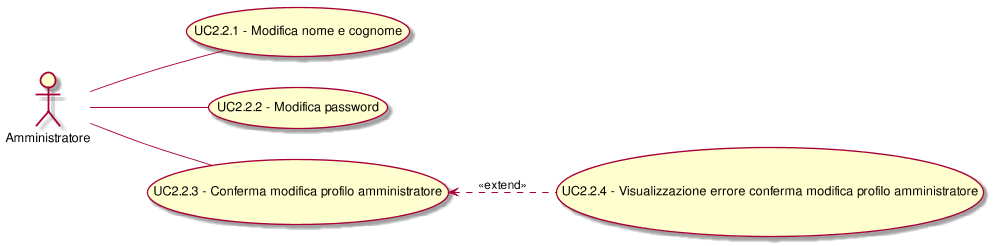
\includegraphics[width=\textwidth,height=\textheight,keepaspectratio]{images/UseCaseUC22.png}
\caption{UC2.2: Gestione profilo amministratore}
\end{figure}
\begin{longtable}{l|p{10cm}}
\rowcolor[gray]{0.8} \multicolumn{2}{c}{} \\
\rowcolor[gray]{0.8} \multicolumn{2}{c}{\textbf{UC2.2 - Gestione profilo amministratore}} \\
\rowcolor[gray]{0.8} \multicolumn{2}{c}{} \\
\hline
&\\
\textbf{Attori} & Amministratore.\\[7pt]
\textbf{Descrizione} & L'amministratore può gestire le impostazioni del proprio profilo tramite le funzionalità  offerte dal sistema.\\[7pt]
\textbf{Precondizione} & L'amministratore si trova nella sezione adibita alla gestione delle impostazioni del proprio profilo.\\[7pt]
\textbf{Postcondizione} & L'amministratore ha usufruito delle funzionalità per gestire le impostazioni del proprio profilo.\\[7pt]
\textbf{Scenario principale} &\begin{enumerate}
\item  L'amministratore può modificare il proprio nome e cognome;
\item  L'amministratore può modificare la propria password;
\item  L'amministratore può confermare le modifiche effettuate.
\end{enumerate}
\\[7pt]
\textbf{Scenari alternativi} & L'amministratore visualizza un messaggio d'errore relativo alla conferma della modifica del profilo.\\[7pt]\hline
\end{longtable}

\subsubsection{UC2.2.1: Modifica nome e cognome}
\label{UC2.2.1}
\begin{longtable}{l|p{10cm}}
\rowcolor[gray]{0.8} \multicolumn{2}{c}{} \\
\rowcolor[gray]{0.8} \multicolumn{2}{c}{\textbf{UC2.2.1 - Modifica nome e cognome}} \\
\rowcolor[gray]{0.8} \multicolumn{2}{c}{} \\
\hline
&\\
\textbf{Attori} & Amministratore.\\[7pt]
\textbf{Descrizione} & L'amministratore può modificare il nome e cognome del suo profilo.\\[7pt]
\textbf{Precondizione} & L'amministratore si trova nella sezione dedicata alla modifica del nome e del cognome del suo profilo.\\[7pt]
\textbf{Postcondizione} & L'amministratore ha modificato il nome e cognome del suo profilo.\\[7pt]
\textbf{Scenario principale} &L'amministratore modifica il nome e cognome del suo profilo.\\[7pt]\hline
\end{longtable}

\subsubsection{UC2.2.2: Modifica password}
\label{UC2.2.2}
\begin{figure}[h]
\centering
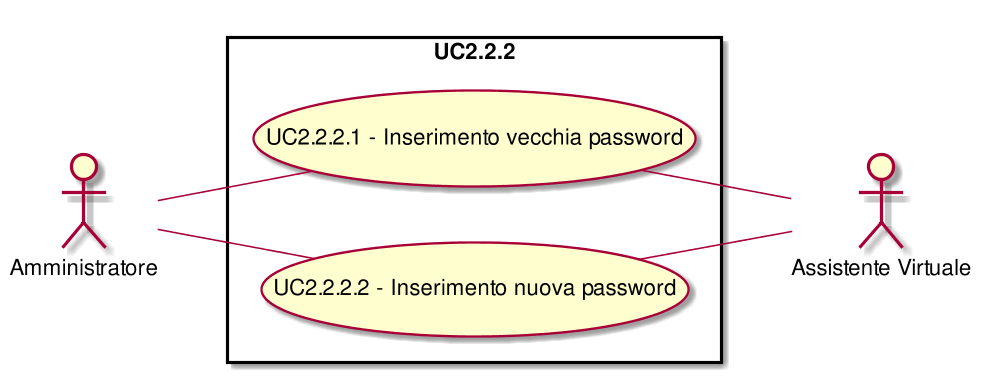
\includegraphics[width=\textwidth,height=\textheight,keepaspectratio]{images/UseCaseUC222.png}
\caption{UC2.2.2: Modifica password}
\end{figure}
\begin{longtable}{l|p{10cm}}
\rowcolor[gray]{0.8} \multicolumn{2}{c}{} \\
\rowcolor[gray]{0.8} \multicolumn{2}{c}{\textbf{UC2.2.2 - Modifica password}} \\
\rowcolor[gray]{0.8} \multicolumn{2}{c}{} \\
\hline
&\\
\textbf{Attori} & Amministratore.\\[7pt]
\textbf{Descrizione} & L'amministratore può modificare la password del suo profilo.\\[7pt]
\textbf{Precondizione} & L'amministratore si trova nella sezione dedicata alla modifica della password del suo profilo.\\[7pt]
\textbf{Postcondizione} & L'amministratore ha modificato la password del suo profilo.\\[7pt]
\textbf{Scenario principale} &\begin{enumerate}
\item  L'attore può inserire la propria vecchia password;
\item  L'attore può inserire una nuova password.
\end{enumerate}
\\[7pt]
\textbf{Scenari alternativi} & L'amministratore non conferma di voler modificare la propria password. L'amministratore viene rimandato alla pagina dedicata alla gestione delle direttive.\\[7pt]\hline
\end{longtable}

\subsubsection{UC2.2.2.1: Inserimento vecchia password}
\label{UC2.2.2.1}
\begin{longtable}{l|p{10cm}}
\rowcolor[gray]{0.8} \multicolumn{2}{c}{} \\
\rowcolor[gray]{0.8} \multicolumn{2}{c}{\textbf{UC2.2.2.1 - Inserimento vecchia password}} \\
\rowcolor[gray]{0.8} \multicolumn{2}{c}{} \\
\hline
&\\
\textbf{Attori} & Amministratore.\\[7pt]
\textbf{Descrizione} & L'amministratore può inserire la vecchia password.\\[7pt]
\textbf{Precondizione} & L'amministratore si trova nella sezione dedicata all'inserimento della vecchia password.\\[7pt]
\textbf{Postcondizione} & L'amministratore ha inserito la vecchia password.\\[7pt]
\textbf{Scenario principale} &L'amministratore inserisce la vecchia password.\\[7pt]\hline
\end{longtable}

\subsubsection{UC2.2.2.2: Inserimento nuova password}
\label{UC2.2.2.2}
\begin{longtable}{l|p{10cm}}
\rowcolor[gray]{0.8} \multicolumn{2}{c}{} \\
\rowcolor[gray]{0.8} \multicolumn{2}{c}{\textbf{UC2.2.2.2 - Inserimento nuova password}} \\
\rowcolor[gray]{0.8} \multicolumn{2}{c}{} \\
\hline
&\\
\textbf{Attori} & Amministratore.\\[7pt]
\textbf{Descrizione} & L'amministratore può inserire la nuova password.\\[7pt]
\textbf{Precondizione} & L'amministratore si trova nella sezione dedicata all'inserimento di una nuova password.\\[7pt]
\textbf{Postcondizione} & L'amministratore inserisce la nuova password.\\[7pt]
\textbf{Scenario principale} &L'amministratore inserisce la nuova password.\\[7pt]\hline
\end{longtable}

\subsubsection{UC2.2.3: Conferma modifica profilo amministratore}
\label{UC2.2.3}
\begin{longtable}{l|p{10cm}}
\rowcolor[gray]{0.8} \multicolumn{2}{c}{} \\
\rowcolor[gray]{0.8} \multicolumn{2}{c}{\textbf{UC2.2.3 - Conferma modifica profilo amministratore}} \\
\rowcolor[gray]{0.8} \multicolumn{2}{c}{} \\
\hline
&\\
\textbf{Attori} & Amministratore.\\[7pt]
\textbf{Descrizione} & L'amministratore può confermare le modifiche al profilo.\\[7pt]
\textbf{Precondizione} & L'amministratore ha inserito i dati necessari alla modifica del profilo.\\[7pt]
\textbf{Postcondizione} & L'amministratore ha modificato il profilo.\\[7pt]
\textbf{Scenario principale} &L'amministratore modifica il profilo.\\[7pt]\hline
\end{longtable}

\subsubsection{UC2.2.4: Visualizzazione errore conferma modifica profilo amministratore }
\label{UC2.2.4}
\begin{longtable}{l|p{10cm}}
\rowcolor[gray]{0.8} \multicolumn{2}{c}{} \\
\rowcolor[gray]{0.8} \multicolumn{2}{c}{\textbf{UC2.2.4 - Visualizzazione errore conferma modifica profilo amministratore }} \\
\rowcolor[gray]{0.8} \multicolumn{2}{c}{} \\
\hline
&\\
\textbf{Attori} & Amministratore.\\[7pt]
\textbf{Descrizione} & L'amministratore può visualizzare un messaggio d'errore se ha comunicato dei dati nulli o non validi per la modifica del profilo d'amministratore.\\[7pt]
\textbf{Precondizione} & Il sistema ha ricevuto dati vuoti o non validi.\\[7pt]
\textbf{Postcondizione} & Il sistema mostra un messaggio d'errore.\\[7pt]
\textbf{Scenario principale} &L'amministratore visualizza un messaggio d'errore.\\[7pt]\hline
\end{longtable}

\newpage\subsection{UC3: Accoglienza ospite}
\label{UC3}
\begin{figure}[h]
\centering
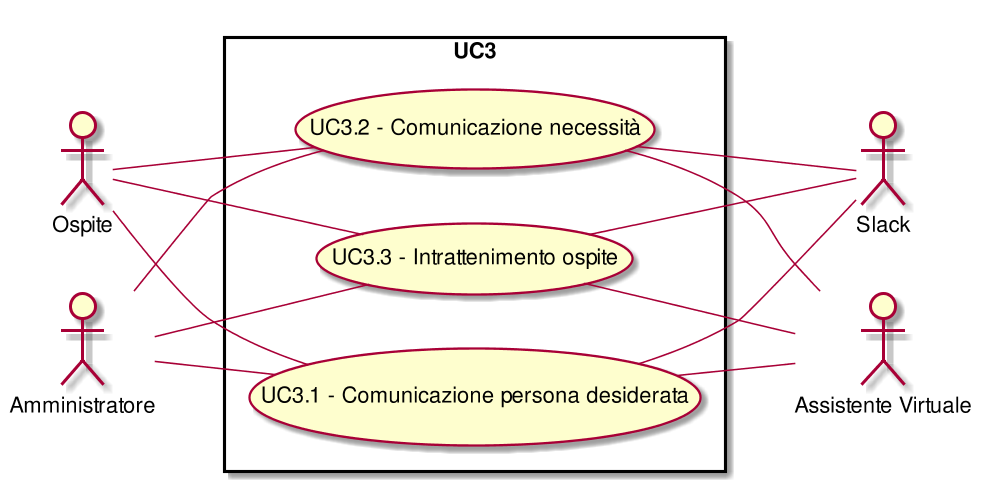
\includegraphics[width=\textwidth,height=\textheight,keepaspectratio]{images/UseCaseUC3.png}
\caption{UC3: Accoglienza ospite}
\end{figure}
\begin{longtable}{l|p{10cm}}
\rowcolor[gray]{0.8} \multicolumn{2}{c}{} \\
\rowcolor[gray]{0.8} \multicolumn{2}{c}{\textbf{UC3 - Accoglienza ospite}} \\
\rowcolor[gray]{0.8} \multicolumn{2}{c}{} \\
\hline
&\\
\textbf{Attori} & Ospite.\\[7pt]
\textbf{Descrizione} & L'ospite può essere accolto dal sistema tramite le funzionalità da esso offerte.\\[7pt]
\textbf{Precondizione} & Il sistema ha riconosciuto l'utente come ospite dell'azienda.\\[7pt]
\textbf{Postcondizione} & L'ospite è stato accolto usufruendo delle funzionalità del sistema.\\[7pt]
\textbf{Scenario principale} &\begin{enumerate}
\item  L'ospite può comunicare la persona desiderata per il suo incontro;
\item  L'ospite può esprimere alcune necessità  particolari riguardanti l'incontro;
\item  L'ospite può essere intrattenuto dal sistema durante l'attesa.
\end{enumerate}
\\[7pt]\hline
\end{longtable}

\subsubsection{UC3.1: Comunicazione persona desiderata}
\label{UC3.1}
\begin{longtable}{l|p{10cm}}
\rowcolor[gray]{0.8} \multicolumn{2}{c}{} \\
\rowcolor[gray]{0.8} \multicolumn{2}{c}{\textbf{UC3.1 - Comunicazione persona desiderata}} \\
\rowcolor[gray]{0.8} \multicolumn{2}{c}{} \\
\hline
&\\
\textbf{Attori} & Ospite.\\[7pt]
\textbf{Descrizione} & L'ospite può comunicare al sistema la persona che desidera incontrare.\\[7pt]
\textbf{Precondizione} & L'ospite si trova nella sezione adibita alla comunicazione della persona desiderata.\\[7pt]
\textbf{Postcondizione} & L'ospite ha comunicato al sistema la persona che vuole incontrare.\\[7pt]
\textbf{Scenario principale} &L'ospite comunica il nome della persona desiderata.\\[7pt]\hline
\end{longtable}

\subsubsection{UC3.2: Comunicazione necessità}
\label{UC3.2}
\begin{figure}[h]
\centering
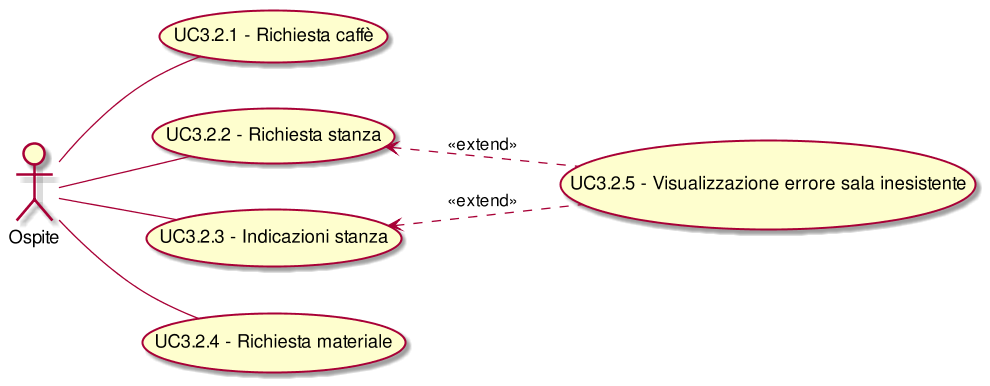
\includegraphics[width=\textwidth,height=\textheight,keepaspectratio]{images/UseCaseUC32.png}
\caption{UC3.2: Comunicazione necessità}
\end{figure}
\begin{longtable}{l|p{10cm}}
\rowcolor[gray]{0.8} \multicolumn{2}{c}{} \\
\rowcolor[gray]{0.8} \multicolumn{2}{c}{\textbf{UC3.2 - Comunicazione necessità}} \\
\rowcolor[gray]{0.8} \multicolumn{2}{c}{} \\
\hline
&\\
\textbf{Attori} & Ospite.\\[7pt]
\textbf{Descrizione} & L'ospite può comunicare al sistema particolari necessità per l'incontro.\\[7pt]
\textbf{Precondizione} & L'ospite si trova nella sezione adibita a comunicare particolari necessità riguardanti l'incontro.\\[7pt]
\textbf{Postcondizione} & L'ospite ha comunicato le necessità.\\[7pt]
\textbf{Scenario principale} &\begin{enumerate}
\item  L'ospite può desiderare un caffè;
\item  L'ospite può chiedere dove si trova una stanza dell'ufficio;
\item  L'ospite può chiedere del materiale particolare per l'incontro.
\end{enumerate}
\\[7pt]\hline
\end{longtable}

\newpage\subsubsection{UC3.2.1: Richiesta caffè}
\label{UC3.2.1}
\begin{longtable}{l|p{10cm}}
\rowcolor[gray]{0.8} \multicolumn{2}{c}{} \\
\rowcolor[gray]{0.8} \multicolumn{2}{c}{\textbf{UC3.2.1 - Richiesta caffè}} \\
\rowcolor[gray]{0.8} \multicolumn{2}{c}{} \\
\hline
&\\
\textbf{Attori} & Ospite.\\[7pt]
\textbf{Descrizione} & L'ospite, nell'attesa, potrebbe desiderare un caffè.\\[7pt]
\textbf{Precondizione} & L'ospite si trova nella sezione adibita a comunicare particolari necessità riguardanti l'incontro.\\[7pt]
\textbf{Postcondizione} & L'ospite ha desiderato un caffè.\\[7pt]
\textbf{Scenario principale} &L'ospite desidera un caffè.\\[7pt]\hline
\end{longtable}

\subsubsection{UC3.2.2: Richiesta stanza}
\label{UC3.2.2}
\begin{longtable}{l|p{10cm}}
\rowcolor[gray]{0.8} \multicolumn{2}{c}{} \\
\rowcolor[gray]{0.8} \multicolumn{2}{c}{\textbf{UC3.2.2 - Richiesta stanza}} \\
\rowcolor[gray]{0.8} \multicolumn{2}{c}{} \\
\hline
&\\
\textbf{Attori} & Ospite.\\[7pt]
\textbf{Descrizione} & L'ospite può chiedere informazioni riguardanti una particolare stanza.\\[7pt]
\textbf{Precondizione} & L'ospite si trova nella sezione adibita a comunicare particolari necessità riguardanti l'incontro.\\[7pt]
\textbf{Postcondizione} & L'ospite ha chiesto informazioni riguardanti una particolare stanza.\\[7pt]
\textbf{Scenario principale} &L'ospite chiede informazioni riguardanti una particolare stanza.\\[7pt]\hline
\end{longtable}

\subsubsection{UC3.2.3: Indicazioni stanza}
\label{UC3.2.3}
\begin{longtable}{l|p{10cm}}
\rowcolor[gray]{0.8} \multicolumn{2}{c}{} \\
\rowcolor[gray]{0.8} \multicolumn{2}{c}{\textbf{UC3.2.3 - Indicazioni stanza}} \\
\rowcolor[gray]{0.8} \multicolumn{2}{c}{} \\
\hline
&\\
\textbf{Attori} & Ospite.\\[7pt]
\textbf{Descrizione} & L'ospite può aver bisogno di dirigersi in qualche stanza e non sapere dove si trova.\\[7pt]
\textbf{Precondizione} & L'ospite si trova nella sezione adibita a comunicare particolari necessità riguardanti l'incontro.\\[7pt]
\textbf{Postcondizione} & L'ospite ha chiesto le indicazioni.\\[7pt]
\textbf{Scenario principale} &L'ospite chiede indicazioni sulla stanza che gli interessa.\\[7pt]
\textbf{Scenari alternativi} & L'ospite potrebbe chiedere indicazioni di una stanza inesistente.\\[7pt]\hline
\end{longtable}

\subsubsection{UC3.2.4: Richiesta materiale}
\label{UC3.2.4}
\begin{longtable}{l|p{10cm}}
\rowcolor[gray]{0.8} \multicolumn{2}{c}{} \\
\rowcolor[gray]{0.8} \multicolumn{2}{c}{\textbf{UC3.2.4 - Richiesta materiale}} \\
\rowcolor[gray]{0.8} \multicolumn{2}{c}{} \\
\hline
&\\
\textbf{Attori} & Ospite.\\[7pt]
\textbf{Descrizione} & L'ospite può aver bisogno di particolare materiale per l'incontro.\\[7pt]
\textbf{Precondizione} & L'ospite si trova nella sezione adibita a comunicare particolari necessità riguardanti l'incontro.\\[7pt]
\textbf{Postcondizione} & L'ospite ha comunicato il materiale desiderato.\\[7pt]
\textbf{Scenario principale} &L'ospite comunica il materiale necessario per l'incontro.\\[7pt]\hline
\end{longtable}

\subsubsection{UC3.2.5: Visualizzazione errore sala inesistente}
\label{UC3.2.5}
\begin{longtable}{l|p{10cm}}
\rowcolor[gray]{0.8} \multicolumn{2}{c}{} \\
\rowcolor[gray]{0.8} \multicolumn{2}{c}{\textbf{UC3.2.5 - Visualizzazione errore sala inesistente}} \\
\rowcolor[gray]{0.8} \multicolumn{2}{c}{} \\
\hline
&\\
\textbf{Attori} & Ospite.\\[7pt]
\textbf{Descrizione} & L'ospite può visualizzare un errore nel caso richieda informazioni su una stanza inesistente.\\[7pt]
\textbf{Precondizione} & Il sistema ha ricevuto dati vuoti o non validi.\\[7pt]
\textbf{Postcondizione} & Il sistema mostra un messaggio d'errore.\\[7pt]
\textbf{Scenario principale} &L'ospite visualizza un messaggio d'errore\\[7pt]\hline
\end{longtable}

\newpage\subsubsection{UC3.3: Intrattenimento ospite}
\label{UC3.3}
\begin{figure}[h]
\centering
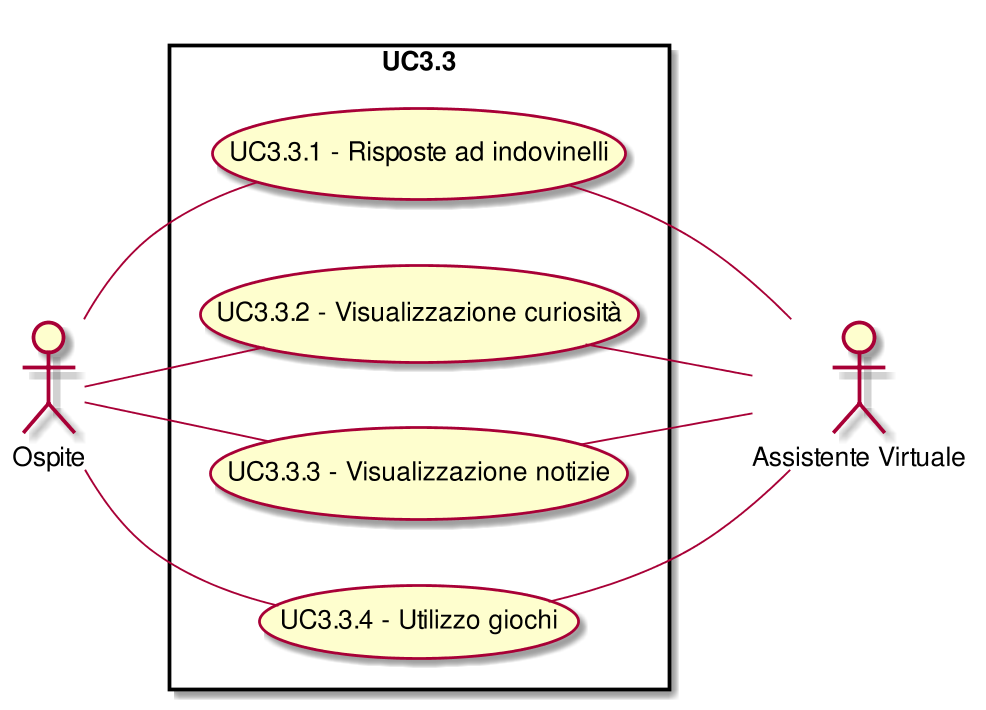
\includegraphics[width=\textwidth,height=\textheight,keepaspectratio]{images/UseCaseUC33.png}
\caption{UC3.3: Intrattenimento ospite}
\end{figure}
\begin{longtable}{l|p{10cm}}
\rowcolor[gray]{0.8} \multicolumn{2}{c}{} \\
\rowcolor[gray]{0.8} \multicolumn{2}{c}{\textbf{UC3.3 - Intrattenimento ospite}} \\
\rowcolor[gray]{0.8} \multicolumn{2}{c}{} \\
\hline
&\\
\textbf{Attori} & Ospite.\\[7pt]
\textbf{Descrizione} & L'ospite può scegliere tra alcuni tipi di intrattenimento forniti dal sistema, mentre attende l'arrivo della persona desiderata.\\[7pt]
\textbf{Precondizione} & L'ospite si trova nella sezione dedicata all'intrattenimento degli ospiti.\\[7pt]
\textbf{Postcondizione} & L'ospite è stato intrattenuto dal sistema.\\[7pt]
\textbf{Scenario principale} &\begin{enumerate}
\item  L'ospite può essere intrattenuto con alcuni indovinelli ai quali deve rispondere;
\item  L'ospite può essere intrattenuto con alcune curiosità di varia natura;3. L'ospite può essere intrattenuto chiedendo di visualizzare alcune notizie di varia natura;
\item  L'ospite può essere intrattenuto con alcuni giochi che il sistema rende disponibili.
\end{enumerate}
\\[7pt]
\textbf{Scenari alternativi} & Dopo un certo lasso di tempo, l'ospite può sollecitare l'arrivo della persona desiderata.\\[7pt]\hline
\end{longtable}

\subsubsection{UC3.3.1: Risposte ad indovinelli}
\label{UC3.3.1}
\begin{longtable}{l|p{10cm}}
\rowcolor[gray]{0.8} \multicolumn{2}{c}{} \\
\rowcolor[gray]{0.8} \multicolumn{2}{c}{\textbf{UC3.3.1 - Risposte ad indovinelli}} \\
\rowcolor[gray]{0.8} \multicolumn{2}{c}{} \\
\hline
&\\
\textbf{Attori} & Ospite.\\[7pt]
\textbf{Descrizione} & L'ospite può rispondere ad alcuni indovinelli fatti dal sistema.\\[7pt]
\textbf{Precondizione} & L'ospite si trova nella sezione dedicata alla risposta degli indovinelli.\\[7pt]
\textbf{Postcondizione} & L'ospite ha risposto agli indovinelli.\\[7pt]
\textbf{Scenario principale} &L'ospite risponde agli indovinelli posti dal sistema.\\[7pt]\hline
\end{longtable}

\subsubsection{UC3.3.2: Visualizzazione curiosità}
\label{UC3.3.2}
\begin{longtable}{l|p{10cm}}
\rowcolor[gray]{0.8} \multicolumn{2}{c}{} \\
\rowcolor[gray]{0.8} \multicolumn{2}{c}{\textbf{UC3.3.2 - Visualizzazione curiosità}} \\
\rowcolor[gray]{0.8} \multicolumn{2}{c}{} \\
\hline
&\\
\textbf{Attori} & Ospite.\\[7pt]
\textbf{Descrizione} & L'ospite può essere intrattenuto dal sistema tramite la visualizzazione di curiosità di vario genere.\\[7pt]
\textbf{Precondizione} & L'ospite si trova nella sezione dedicata alla visualizzazione delle curiosità.\\[7pt]
\textbf{Postcondizione} & L'ospite ha visualizzato alcune curiosità.\\[7pt]
\textbf{Scenario principale} &L'ospite visualizza le curiosità fornite dal sistema.\\[7pt]\hline
\end{longtable}

\subsubsection{UC3.3.3: Visualizzazione notizie}
\label{UC3.3.3}
\begin{longtable}{l|p{10cm}}
\rowcolor[gray]{0.8} \multicolumn{2}{c}{} \\
\rowcolor[gray]{0.8} \multicolumn{2}{c}{\textbf{UC3.3.3 - Visualizzazione notizie}} \\
\rowcolor[gray]{0.8} \multicolumn{2}{c}{} \\
\hline
&\\
\textbf{Attori} & Ospite.\\[7pt]
\textbf{Descrizione} & L'ospite può essere intrattenuto chiedendo di visualizzare le ultime notizie riguardanti categorie di vario genere.\\[7pt]
\textbf{Precondizione} & L'ospite si trova nella sezione dedicata alla visualizzazione delle notizie.\\[7pt]
\textbf{Postcondizione} & L'ospite ha visualizzato le notizie da lui richieste.\\[7pt]
\textbf{Scenario principale} &L'ospite visualizza le notizie riguardanti la categoria richiesta.\\[7pt]\hline
\end{longtable}

\subsubsection{UC3.3.4: Utilizzo giochi}
\label{UC3.3.4}
\begin{longtable}{l|p{10cm}}
\rowcolor[gray]{0.8} \multicolumn{2}{c}{} \\
\rowcolor[gray]{0.8} \multicolumn{2}{c}{\textbf{UC3.3.4 - Utilizzo giochi}} \\
\rowcolor[gray]{0.8} \multicolumn{2}{c}{} \\
\hline
&\\
\textbf{Attori} & Ospite.\\[7pt]
\textbf{Descrizione} & L'ospite può essere intrattenuto tramite alcuni giochi forniti dal sistema.\\[7pt]
\textbf{Precondizione} & L'ospite si trova nella sezione dedicata ai giochi.\\[7pt]
\textbf{Postcondizione} & L'ospite ha interagito con i giochi forniti dal sistema.\\[7pt]
\textbf{Scenario principale} &L'ospite interagisce con i giochi forniti dal sistema.\\[7pt]\hline
\end{longtable}

\subsection{UC4: Comunicazione nome azienda}
\label{UC4}
\begin{longtable}{l|p{10cm}}
\rowcolor[gray]{0.8} \multicolumn{2}{c}{} \\
\rowcolor[gray]{0.8} \multicolumn{2}{c}{\textbf{UC4 - Comunicazione nome azienda}} \\
\rowcolor[gray]{0.8} \multicolumn{2}{c}{} \\
\hline
&\\
\textbf{Attori} & Utente.\\[7pt]
\textbf{Descrizione} & L'utente può comunicare il nome dell'azienda di cui fa parte.\\[7pt]
\textbf{Precondizione} & L'utente appartiene ad una azienda.\\[7pt]
\textbf{Postcondizione} & L'utente ha comunicato al sistema il nome dell'azienda di cui fa parte.\\[7pt]
\textbf{Scenario principale} &L'utente comunica il nome della propria azienda di provenienza.\\[7pt]\hline
\end{longtable}

\subsection{UC5: Comunicazione non comprensibile}
\label{UC5}
\begin{longtable}{l|p{10cm}}
\rowcolor[gray]{0.8} \multicolumn{2}{c}{} \\
\rowcolor[gray]{0.8} \multicolumn{2}{c}{\textbf{UC5 - Comunicazione non comprensibile}} \\
\rowcolor[gray]{0.8} \multicolumn{2}{c}{} \\
\hline
&\\
\textbf{Attori} & Amministratore, Ospite, Utente.\\[7pt]
\textbf{Descrizione} & Il sistema richiederà all'utente una chiarimento nel caso in cui non riesca a interpretare la sua risposta.\\[7pt]
\textbf{Precondizione} & Il sistema non è riuscito ad interpretare una comunicazione dell'utente.\\[7pt]
\textbf{Postcondizione} & Il sistema comunica l'errore richiedendo nuovamente l'informazione all'utente.\\[7pt]
\textbf{Scenario principale} &L'utente comunica nuovamente l'informazione non compresa dal sistema.\\[7pt]\hline
\end{longtable}

\subsection{UC6: Scadenza timeout input}
\label{UC6}
\begin{longtable}{l|p{10cm}}
\rowcolor[gray]{0.8} \multicolumn{2}{c}{} \\
\rowcolor[gray]{0.8} \multicolumn{2}{c}{\textbf{UC6 - Scadenza timeout input}} \\
\rowcolor[gray]{0.8} \multicolumn{2}{c}{} \\
\hline
&\\
\textbf{Attori} & Amministratore, Ospite, Utente.\\[7pt]
\textbf{Descrizione} & L'utente, per ogni interazione con il sistema, ha un tempo limitato di risposta. Scaduto questo lasso di tempo l'utente visualizzerà un opportuno messaggio, attraverso il quale potrà tornare alla schermata precedente.\\[7pt]
\textbf{Precondizione} & L'utente non ha interagito con il sistema entro il tempo prestabilito di risposta.\\[7pt]
\textbf{Postcondizione} & L'utente ha visualizzato il messaggio oppure il sistema si è disattivato.\\[7pt]
\textbf{Scenario principale} &L'utente visualizza un messaggio opportuno. \\[7pt]
\textbf{Scenari alternativi} & Nel caso in cui l'utente non confermi la sua presenza il sistema si disattiva.\\[7pt]\hline
\end{longtable}

\newpage\subsection{UC7: Accesso funzionalità super amministratore}
\label{UC7}
\begin{figure}[h]
\centering
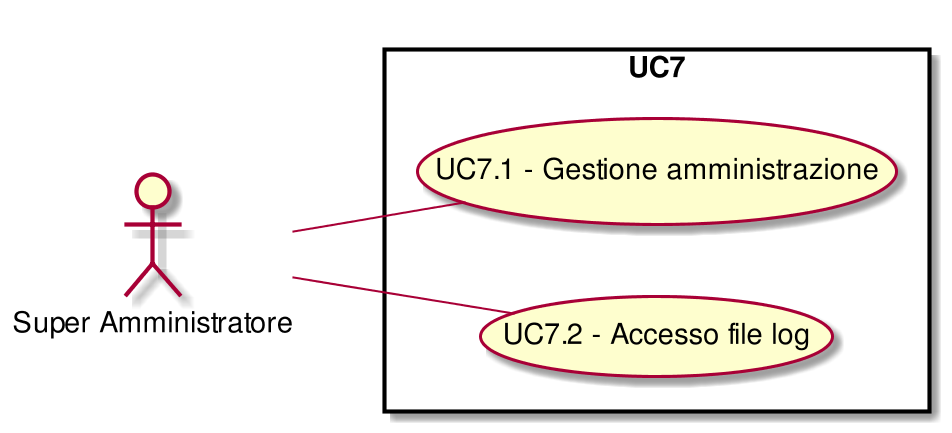
\includegraphics[width=\textwidth,height=\textheight,keepaspectratio]{images/UseCaseUC7.png}
\caption{UC7: Accesso funzionalità super amministratore}
\end{figure}
\begin{longtable}{l|p{10cm}}
\rowcolor[gray]{0.8} \multicolumn{2}{c}{} \\
\rowcolor[gray]{0.8} \multicolumn{2}{c}{\textbf{UC7 - Accesso funzionalità super amministratore}} \\
\rowcolor[gray]{0.8} \multicolumn{2}{c}{} \\
\hline
&\\
\textbf{Attori} & Super Amministratore.\\[7pt]
\textbf{Descrizione} & Il super amministratore può gestire gli amministratori ed accedere ai file log.\\[7pt]
\textbf{Precondizione} & Il super amministratore si trova nella sezione adibita alla gestione.\\[7pt]
\textbf{Postcondizione} & Il super amministratore ha usufruito delle funzionalità di gestione.\\[7pt]
\textbf{Scenario principale} &\begin{enumerate}
\item  Il super amministratore può gestire gli amministratori del sistema; 
\item  Il super amministratore può accedere ai file log.
\end{enumerate}
\\[7pt]\hline
\end{longtable}

\newpage\subsubsection{UC7.1: Gestione amministrazione}
\label{UC7.1}
\begin{figure}[h]
\centering
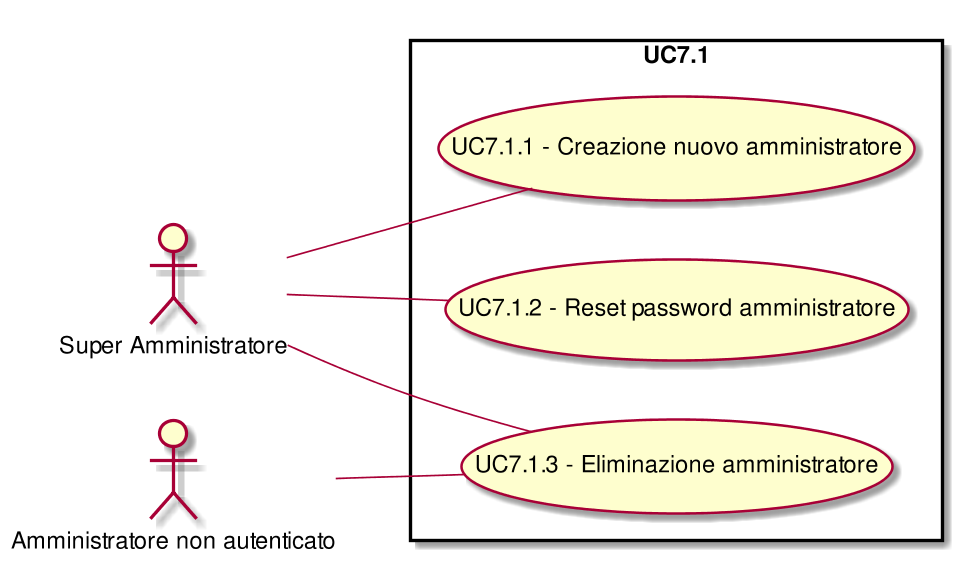
\includegraphics[width=\textwidth,height=\textheight,keepaspectratio]{images/UseCaseUC71.png}
\caption{UC7.1: Gestione amministrazione}
\end{figure}
\begin{longtable}{l|p{10cm}}
\rowcolor[gray]{0.8} \multicolumn{2}{c}{} \\
\rowcolor[gray]{0.8} \multicolumn{2}{c}{\textbf{UC7.1 - Gestione amministrazione}} \\
\rowcolor[gray]{0.8} \multicolumn{2}{c}{} \\
\hline
&\\
\textbf{Attori} & Super Amministratore.\\[7pt]
\textbf{Descrizione} & Il super amministratore può gestire gli amministratori del sistema.\\[7pt]
\textbf{Precondizione} & Il super amministratore si trova nella sezione per gestire gli amministratori.\\[7pt]
\textbf{Postcondizione} & Il super amministratore ha usufruito delle funzionalità per gestire gli amministratori.\\[7pt]
\textbf{Scenario principale} &\begin{enumerate}
\item  Il super amministratore può creare un nuovo amministratore;
\item  Il super amministratore può resettare la password degli amministratori;
\item  Il super amministratore può revocare i privilegi degli amministratori.
\end{enumerate}
\\[7pt]\hline
\end{longtable}

\newpage\subsubsection{UC7.1.1: Creazione nuovo amministratore}
\label{UC7.1.1}
\begin{figure}[h]
\centering
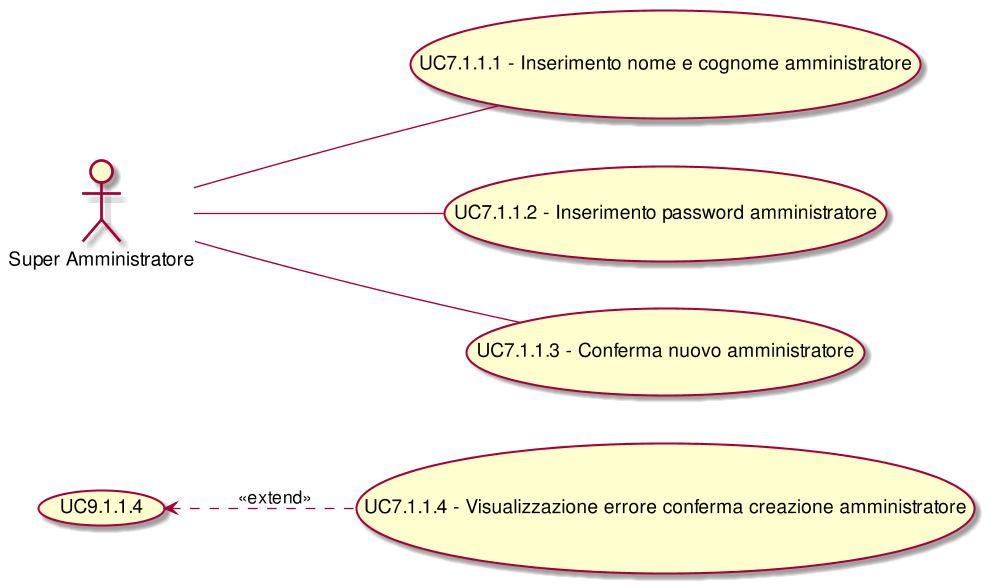
\includegraphics[width=\textwidth,height=\textheight,keepaspectratio]{images/UseCaseUC711.png}
\caption{UC7.1.1: Creazione nuovo amministratore}
\end{figure}
\begin{longtable}{l|p{10cm}}
\rowcolor[gray]{0.8} \multicolumn{2}{c}{} \\
\rowcolor[gray]{0.8} \multicolumn{2}{c}{\textbf{UC7.1.1 - Creazione nuovo amministratore}} \\
\rowcolor[gray]{0.8} \multicolumn{2}{c}{} \\
\hline
&\\
\textbf{Attori} & Super Amministratore.\\[7pt]
\textbf{Descrizione} & Il super amministratore può creare un nuovo amministratore.\\[7pt]
\textbf{Precondizione} & Il super amministratore si trova nella sezione per creare un nuovo amministratore.\\[7pt]
\textbf{Postcondizione} & Il super amministratore ha creato un nuovo amministratore.\\[7pt]
\textbf{Scenario principale} &\begin{enumerate}
\item  Il super amministratore può inserire nome e cognome dell'amministratore;
\item  Il super amministratore può inserire la password dell'amministratore;
\item  Il super amministratore può confermare il nuovo amministratore.
\end{enumerate}
\\[7pt]
\textbf{Scenari alternativi} & Il super amministratore visualizza un messaggio d'errore relativo alla conferma della creazione dell'amministratore.\\[7pt]\hline
\end{longtable}

\subsubsection{UC7.1.1.1: Inserimento nome e cognome amministratore}
\label{UC7.1.1.1}
\begin{longtable}{l|p{10cm}}
\rowcolor[gray]{0.8} \multicolumn{2}{c}{} \\
\rowcolor[gray]{0.8} \multicolumn{2}{c}{\textbf{UC7.1.1.1 - Inserimento nome e cognome amministratore}} \\
\rowcolor[gray]{0.8} \multicolumn{2}{c}{} \\
\hline
&\\
\textbf{Attori} & Super Amministratore.\\[7pt]
\textbf{Descrizione} & Il super amministratore può inserire nome e cognome del nuovo amministratore.\\[7pt]
\textbf{Precondizione} & Il super amministratore si trova nella sezione per creare un nuovo amministratore. \\[7pt]
\textbf{Postcondizione} & Il super amministratore ha inserito nome e cognome del nuovo amministratore.\\[7pt]
\textbf{Scenario principale} &Il super amministratore inserisce nome e cognome di un nuovo amministratore.\\[7pt]\hline
\end{longtable}

\subsubsection{UC7.1.1.2: Inserimento password amministratore}
\label{UC7.1.1.2}
\begin{longtable}{l|p{10cm}}
\rowcolor[gray]{0.8} \multicolumn{2}{c}{} \\
\rowcolor[gray]{0.8} \multicolumn{2}{c}{\textbf{UC7.1.1.2 - Inserimento password amministratore}} \\
\rowcolor[gray]{0.8} \multicolumn{2}{c}{} \\
\hline
&\\
\textbf{Attori} & Super Amministratore.\\[7pt]
\textbf{Descrizione} & Il super amministratore può inserire la password di un nuovo amministratore.\\[7pt]
\textbf{Precondizione} & Il super amministratore si trova nella sezione per creare un nuovo amministratore. \\[7pt]
\textbf{Postcondizione} & Il super amministratore ha inserito la password del nuovo amministratore.\\[7pt]
\textbf{Scenario principale} &Il super amministratore inserisce la password per il nuovo amministratore.\\[7pt]\hline
\end{longtable}

\subsubsection{UC7.1.1.3: Conferma creazione nuovo amministratore}
\label{UC7.1.1.3}
\begin{longtable}{l|p{10cm}}
\rowcolor[gray]{0.8} \multicolumn{2}{c}{} \\
\rowcolor[gray]{0.8} \multicolumn{2}{c}{\textbf{UC7.1.1.3 - Conferma creazione nuovo amministratore}} \\
\rowcolor[gray]{0.8} \multicolumn{2}{c}{} \\
\hline
&\\
\textbf{Attori} & Super Amministratore.\\[7pt]
\textbf{Descrizione} & Il super amministratore può confermare i dati inseriti per la creazione di un nuovo amministratore.\\[7pt]
\textbf{Precondizione} & Il super amministratore si trova nella sezione per creare un nuovo amministratore. \\[7pt]
\textbf{Postcondizione} & Il super amministratore ha confermato la creazione del nuovo amministratore.\\[7pt]
\textbf{Scenario principale} &Il super amministratore conferma la creazione di un nuovo amministratore.\\[7pt]
\textbf{Scenari alternativi} & Il super amministratore non conferma di voler creare il nuovo amministratore. Il super amministratore viene rimandato alla pagina dedicata alla gestione degli amministratori.\\[7pt]\hline
\end{longtable}

\subsubsection{UC7.1.1.4: Visualizzazione errore conferma creazione amministratore}
\label{UC7.1.1.4}
\begin{longtable}{l|p{10cm}}
\rowcolor[gray]{0.8} \multicolumn{2}{c}{} \\
\rowcolor[gray]{0.8} \multicolumn{2}{c}{\textbf{UC7.1.1.4 - Visualizzazione errore conferma creazione amministratore}} \\
\rowcolor[gray]{0.8} \multicolumn{2}{c}{} \\
\hline
&\\
\textbf{Attori} & Super Amministratore.\\[7pt]
\textbf{Descrizione} & Il super amministratore può visualizzare un messaggio d'errore se ha comunicato dei dati nulli o non validi per la creazione di un nuovo amministratore.\\[7pt]
\textbf{Precondizione} & Il sistema ha ricevuto dati vuoti o non validi.\\[7pt]
\textbf{Postcondizione} & Il sistema mostra un messaggio d'errore.\\[7pt]
\textbf{Scenario principale} &Il super amministratore visualizza un messaggio d'errore.\\[7pt]\hline
\end{longtable}

\subsubsection{UC7.1.2: Reset password amministratore}
\label{UC7.1.2}
\begin{figure}[h]
\centering
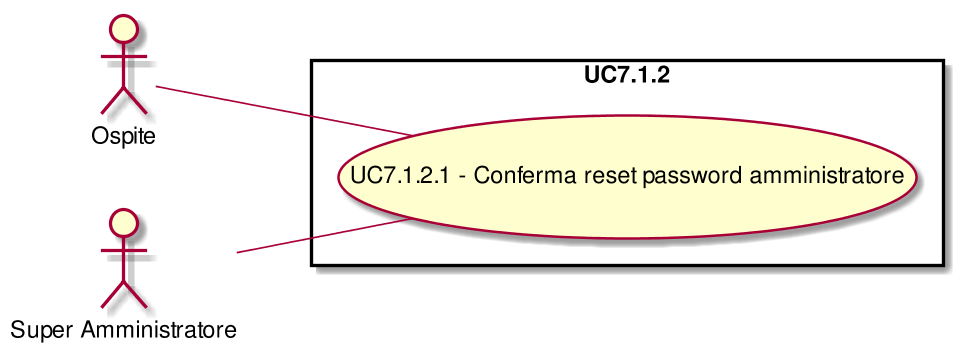
\includegraphics[width=\textwidth,height=\textheight,keepaspectratio]{images/UseCaseUC712.png}
\caption{UC7.1.2: Reset password amministratore}
\end{figure}
\begin{longtable}{l|p{10cm}}
\rowcolor[gray]{0.8} \multicolumn{2}{c}{} \\
\rowcolor[gray]{0.8} \multicolumn{2}{c}{\textbf{UC7.1.2 - Reset password amministratore}} \\
\rowcolor[gray]{0.8} \multicolumn{2}{c}{} \\
\hline
&\\
\textbf{Attori} & Super Amministratore.\\[7pt]
\textbf{Descrizione} & Il super amministratore può resettare la password dell'amministratore.\\[7pt]
\textbf{Precondizione} & Il super amministratore si trova nella sezione per resettare la password di un amministratore.\\[7pt]
\textbf{Postcondizione} & Il super amministratore ha resettato la password dell'amministratore.\\[7pt]
\textbf{Scenario principale} &\begin{enumerate}
\item  Il super amministratore può inserire la nuova password dell'amministratore;
\item  il super amministratore può confermare la nuova password dell'amministratore;
\item  il super amministratore può confermare il reset della password.
\end{enumerate}
\\[7pt]
\textbf{Scenari alternativi} & Il super amministratore visualizza un messaggio d'errore relativo al reset della password dell'amministratore.\\[7pt]\hline
\end{longtable}

\subsubsection{UC7.1.2.1: Conferma reset password amministratore}
\label{UC7.1.2.1}
\begin{longtable}{l|p{10cm}}
\rowcolor[gray]{0.8} \multicolumn{2}{c}{} \\
\rowcolor[gray]{0.8} \multicolumn{2}{c}{\textbf{UC7.1.2.1 - Conferma reset password amministratore}} \\
\rowcolor[gray]{0.8} \multicolumn{2}{c}{} \\
\hline
&\\
\textbf{Attori} & Super Amministratore.\\[7pt]
\textbf{Descrizione} & Il super amministratore può confermare il reset della password.\\[7pt]
\textbf{Precondizione} & Il super amministratore si trova nella sezione per confermare il reset della password dell'amministratore.\\[7pt]
\textbf{Postcondizione} & Il super amministratore ha confermato il reset della password dell'amministratore.\\[7pt]
\textbf{Scenario principale} &Il super amministratore conferma il reset della password dell'amministratore.\\[7pt]
\textbf{Scenari alternativi} & Il super amministratore non conferma di voler resettare la password dell'amministratore. Il super amministratore viene rimandato alla pagina dedicata alla gestione degli amministratori.\\[7pt]\hline
\end{longtable}

\subsubsection{UC7.1.3: Eliminazione amministratore}
\label{UC7.1.3}
\begin{figure}[h]
\centering
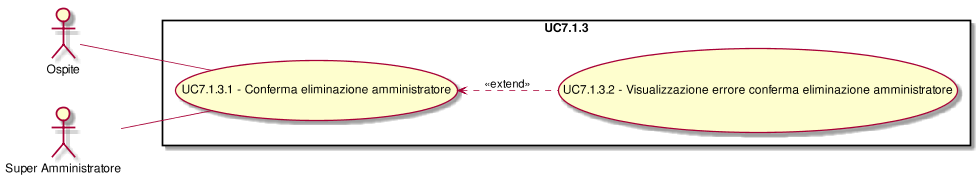
\includegraphics[width=\textwidth,height=\textheight,keepaspectratio]{images/UseCaseUC713.png}
\caption{UC7.1.3: Eliminazione amministratore}
\end{figure}
\begin{longtable}{l|p{10cm}}
\rowcolor[gray]{0.8} \multicolumn{2}{c}{} \\
\rowcolor[gray]{0.8} \multicolumn{2}{c}{\textbf{UC7.1.3 - Eliminazione amministratore}} \\
\rowcolor[gray]{0.8} \multicolumn{2}{c}{} \\
\hline
&\\
\textbf{Attori} & Super Amministratore.\\[7pt]
\textbf{Descrizione} & Il super amministratore può rimuovere un amministratore dal sistema\\[7pt]
\textbf{Precondizione} & Il super amministratore si trova nella sezione per l'eliminazione di un amministratore.\\[7pt]
\textbf{Postcondizione} & Il super amministratore ha eliminato un amministratore dal sistema.\\[7pt]
\textbf{Scenario principale} &\begin{enumerate}
\item  Il super amministratore può eliminare un amministratore;
\item  il super amministratore può confermare l'eliminazione dell'amministratore.
\end{enumerate}
\\[7pt]
\textbf{Scenari alternativi} & Il super amministratore visualizza un messaggio d'errore relativo alla revoca dei privilegi dell'amministratore.\\[7pt]\hline
\end{longtable}

\subsubsection{UC7.1.3.1: Conferma eliminazione amministratore}
\label{UC7.1.3.1}
\begin{longtable}{l|p{10cm}}
\rowcolor[gray]{0.8} \multicolumn{2}{c}{} \\
\rowcolor[gray]{0.8} \multicolumn{2}{c}{\textbf{UC7.1.3.1 - Conferma eliminazione amministratore}} \\
\rowcolor[gray]{0.8} \multicolumn{2}{c}{} \\
\hline
&\\
\textbf{Attori} & Super Amministratore.\\[7pt]
\textbf{Descrizione} & Il super amministratore può confermare l'eliminazione di un amministratore.\\[7pt]
\textbf{Precondizione} & Il super amministratore ha comunicato l'amministratore che vuole eliminare.\\[7pt]
\textbf{Postcondizione} & Il super amministratore ha eliminato un amministratore\\[7pt]
\textbf{Scenario principale} &Il super amministratore conferma di volere eliminare un amministratore.\\[7pt]
\textbf{Scenari alternativi} & Il super amministratore non conferma di voler eliminare l'amministratore . Il super amministratore viene rimandato alla pagina dedicata alla gestione degli amministratori.\\[7pt]\hline
\end{longtable}

\subsubsection{UC7.1.3.2: Visualizzazione errore conferma eliminazione amministratore}
\label{UC7.1.3.2}
\begin{longtable}{l|p{10cm}}
\rowcolor[gray]{0.8} \multicolumn{2}{c}{} \\
\rowcolor[gray]{0.8} \multicolumn{2}{c}{\textbf{UC7.1.3.2 - Visualizzazione errore conferma eliminazione amministratore}} \\
\rowcolor[gray]{0.8} \multicolumn{2}{c}{} \\
\hline
&\\
\textbf{Attori} & Super Amministratore.\\[7pt]
\textbf{Descrizione} & L'amministratore può visualizzare un messaggio d'errore se ha comunicato dei dati nulli o non validi per l'eliminazione di un amministratore.\\[7pt]
\textbf{Precondizione} & Il sistema ha ricevuto dati vuoti o non validi.\\[7pt]
\textbf{Postcondizione} & Il sistema mostra un messaggio d'errore.\\[7pt]
\textbf{Scenario principale} &Il super amministratore visualizza un messaggio d'errore.\\[7pt]\hline
\end{longtable}

\subsubsection{UC7.2: Accesso file log}
\label{UC7.2}
\begin{longtable}{l|p{10cm}}
\rowcolor[gray]{0.8} \multicolumn{2}{c}{} \\
\rowcolor[gray]{0.8} \multicolumn{2}{c}{\textbf{UC7.2 - Accesso file log}} \\
\rowcolor[gray]{0.8} \multicolumn{2}{c}{} \\
\hline
&\\
\textbf{Attori} & Super Amministratore;\\[7pt]
\textbf{Descrizione} & Il super amministratore può accedere ai file \gl{log}.\\[7pt]
\textbf{Precondizione} & Il super amministratore si trova nella sezione adibita alla visualizzazione dei file \gl{log}.\\[7pt]
\textbf{Postcondizione} & Il super amministratore ha fatto accesso ai file \gl{log}\\[7pt]
\textbf{Scenario principale} & Il super amministratore accede e visualizza i file \gl{log}.\\[7pt]\hline
\end{longtable}

\newpage\subsection{UC8: Inserimento password amministrazione}
\label{UC8}
\begin{longtable}{l|p{10cm}}
\rowcolor[gray]{0.8} \multicolumn{2}{c}{} \\
\rowcolor[gray]{0.8} \multicolumn{2}{c}{\textbf{UC8 - Inserimento password amministrazione}} \\
\rowcolor[gray]{0.8} \multicolumn{2}{c}{} \\
\hline
&\\
\textbf{Attori} & Utente.\\[7pt]
\textbf{Descrizione} & L'utente può fornire la propria password di amministrazione. Nel caso in cui la password fornita sia sbagliata, il sistema la chiederà nuovamente.\\[7pt]
\textbf{Precondizione} & Il sistema ha riconosciuto l'utente come uno degli amministratori del sistema\\[7pt]
\textbf{Postcondizione} & L'utente ha fornito la password di amministrazione del sistema\\[7pt]
\textbf{Scenario principale} &1. L'utente fornisce la propria password di amministrazione\\[7pt]
\textbf{Scenari alternativi} & Nel caso in cui la password fornita non sia valida viene richiesto all'utente di inserire nuovamente la password.\\[7pt]\hline
\end{longtable}

